\section{The Quantum Abstract Machine:  Syntax and Semantics} \label{sec:qam}

\begin{figure}[t]
{\small
  \[\begin{array}{llcl} 
      \texttt{Variable} & x,y \\
      \texttt{Probability} & p &\in &\Rs\\
      \texttt{Quantum Message} & m &\in& \mathbb{M}\\
      \texttt{Classical Message} & m_l,m_r &\in& \mathbb{M}_{l\mid r}\\
    \texttt{Quantum Channel} & c &\in& \Ls\\
    \texttt{Classical Channel} & \overline{c} &\in& \Ls\\
    \texttt{Time Stamp} & t &\in& \mathbb{T}\\
\ignore{
    \texttt{Timed Label} & \alpha^t &::=& \qsend{p}{c}{m}^{t}\\
    \texttt{Label} & \iota &::=& c.m \mid p.c.m \mid \alpha^t \mid \emptyset\\
}
      \texttt{Configuration} & C & \\
      \texttt{Rule} & \rules & ::= & C \xrightarrow{\alpha} C 
    \end{array}
  \]
}
\caption{Quantum Abstract Machine Syntax Table}
  \label{fig:q-pi-syntax}
\end{figure}

Here, we first describe a system models single location communication, via the quantum teleportation and GHZ channel building algorithms in \Cref{sec:qamsyntax}, then a system models multiple location communication, via quantum routing in \Cref{sec:qamsyntax1},
and formalize an evaluation framework based on the model in \Cref{sec:qamsemantics1}.

We define QAM system to represent the transitions for any quantum network protocols, which allows programmers to define initial configurations, representing the initial programs and process environment, as well as user-definable transition rules, guiding how configurations are transitioned. A QAM system is a structure $(\Ms,\Ls,\Ts,\overline{\rules})$,
where $\Ms$ is a set of messages;
$\Ls$ is a set of channels;
$\Ts$ is a set of time stamps that forms a linear order ($<$) with $0$ being the minimum;
and $\overline{\rules}$ is a finite set of rules for guiding how configurations are transitioned. 
Any rule has the form $C_1 \xrightarrow{\alpha} C_2$, referring to that we transition configuration $C_1$ to $C_2$ via a label $\alpha$, being either emptily internal ($\emptyset$), a pair $c.m$, a triple $p.c.m$, or a quadruple $(p.c.m)^t$, where $c$ is the channel for communication, $m$ is a possibly quantum message, $p$ is the success rate of the message delivery, and $t$ is the initial time stamp of the message. In QAM, rules are not allowed to associated with side conditions, and we provide special ways of such definitions, explained in \Cref{sec:qamsyntax1}.

The execution in QAM is with respect to a QAM system $(\Ms,\Ls,\Ts,\overline{\rules})$ and an initial configuration $C$ that defines the input program and initial process environment.
If we collect the free metavariables ($\cn{FV}(-)$) appearing in a configuration and rule, 
the initial configuration $C$ is a \textit{ground term} without any metavariables ($\cn{FV}(C)=\emptyset$);
while $\cn{FV}(\alpha) \cup \cn{FV}(C_2)\subseteq \cn{FV}(C_1)$ for every rule $C_1 \xrightarrow{\alpha} C_2$, which is the well-formedness assumption for a QAM system.
We can define the transitions in a QAM system as follows:

\begin{definition}\label{def:labeledsystem}\rm[One QAM Transition Step]
Given a QAM system $\Cs=(\Ms,\Ls,\Ts,\overline{\rules})$ and a ground term initial configuration $C$, a transition step defining for a rule $C_1 \xrightarrow{\alpha} C_2 \in \overline{\rules}$ on $C$ is given as:
\begin{itemize}
\item There is a substitution $\sigma$ mapping every metavariable in $C_1$ to a term, such that $\sigma(C_1)=C$, where we substitute metavariables $x$ in $C_1$ with the mapped terms as $\sigma(x)$.
\item The result label and configuration by applying the rule is $\sigma(\alpha)$ and $\sigma(C_2)$.
\end{itemize}
\end{definition}

\Cref{def:labeledsystem} provides an abstraction of transitions in QAM, where the details configurations and rules are parameterized as some abstract objects.

\subsection{Single Location Communication} \label{sec:qamsyntax}


\begin{figure}[t]
{\small
$\textcolor{blue}{\text{Syntax:}}\\$
  \[\begin{array}{llcl} 
      \texttt{Process} & P,Q & ::= & 0 \mid \down{c}{P}\mid \send{m}{x}{P} \mid \rev {x}{P} \mid \csend{\overline{c}}{m_{l\mid r}}{P}\mid\crev{\overline{c}}{x}{P} \\[0.2em]
    &&\mid& \parp{P}{Q}\mid \comp{P} \mid\parll{P}{c}{R} \mid \parl{P}{R} \mid \mer{m_l}{x}{m_r}{P}\\[1em]
    \texttt{Multi-Process} & R & ::= & \scell{\overline{P}} \mid \pscell{P}{\overline{Q}}\\[0.2em]
      \textcolor{red}{\texttt{Configuration First Pattern}} & \textcolor{red}{C} & \textcolor{red}{::=} & \textcolor{red}{\overline{P}}
    \end{array}
  \]

$\textcolor{blue}{\text{Semantics:}}\\$
  \begin{mathpar}
   \inferrule[Self]{}
       {\down{c}{\send{m}{x}{P}} \longrightarrow \parll{\send{m}{x}{P}}{c}{\scell{\emptyset}}}

   \inferrule[Cohere]{}
       { \pard{\parll{P}{c}{\scell{...}}}{\down{c}{Q}} \longrightarrow \parll{P}{c}{\scell{\pard{Q}{...}}}}

   \inferrule[Decohere]{}
       {\scell{\pard{Q}{...}} \longrightarrow \pard{{\scell{...}}}{Q} }

   \inferrule[Clean]{}
       {\pscell{Q}{\emptyset} \longrightarrow Q}

   \inferrule[ToCom]{}
       { \scell{\pard{\rev{x}{Q}}{...}} \longrightarrow \pscell{\rev{x}{Q}}{...}}

   \inferrule[Measure]{}
       {\parll{P}{c}{R} \xrightarrow{c} \parl{P[\overline{c}/c]}{R[\overline{c}/c]}}

   \inferrule[ID]{}
       {\pard{0}{P} \longrightarrow P}

   \inferrule[QCom]{}
       {\parl{\send{m}{x}{P}}{\pscell{\rev{y}{P'}}{\overline{Q}}}
               \xrightarrow{m} \pard{\pard{P[m_l/x]}{P'[m_r/y]}}{\overline{Q}}}

  \inferrule[Com]{}
      { \pard{\csend{\overline{c}}{m_l}{P}}{\crev{c}{x}{Q}}
           \longrightarrow \pard{P}{Q[m_l/x]}}

  \inferrule[Recover]{}
      { \mer{m_l}{x}{m_r}{P} \xrightarrow{m_l\wr m_r} P[m/x]}

  \inferrule[CL]{}
      {\parp{P}{Q} \longrightarrow P}

  \inferrule[CR]{}
      {\parp{P}{Q} \longrightarrow Q}

   \inferrule[MT]{}
       {\comp{P} \longrightarrow \pard{P}{\comp{P}}}
      
   \inferrule[NT]{}
       {\comp{P} \longrightarrow 0}
  \end{mathpar}
}
\caption{Single-party communication syntax and semantics}
  \label{fig:q-pi-semantics1}
\end{figure}

\begin{figure}[t]
{\small
\[
\begin{array}{lll}
&
\pard{\down{c}{\send{m}{x}{\csend{c}{x}{0}}}}{
\down{c}{\rev{y}{\crev{c}{u}{\mer{u}{v}{y}{0}}}}
}
&
\\[1em]
\longrightarrow
&
\pard{\parll{\send{m}{x}{\csend{c}{x}{0}}}{c}{\scell{\emptyset}}}
{\down{c}{\rev{y}{\crev{c}{u}{\mer{u}{v}{y}{0}}}}}
&
(\rulelab{Self})
\\[1em]
\longrightarrow
&
\parll{\send{m}{x}{\csend{c}{x}{0}}}{c}{\scell{\rev{y}{\crev{c}{u}{\mer{u}{v}{y}{0}}}}}
&
(\rulelab{Cohere})
\\[1em]
\longrightarrow
&
\parll{\send{m}{x}{\csend{c}{x}{0}}}{c}{\pscell{\rev{y}{\crev{c}{u}{\mer{u}{v}{y}{0}}}}{\emptyset}}
&
(\rulelab{ToCom})
\\[1em]
\longrightarrow
&
\parll{\send{m}{x}{\csend{c}{x}{0}}}{c}{\rev{y}{\crev{c}{u}{\mer{u}{v}{y}{0}}}}
&
(\rulelab{Clean})
\\[1em]
\xrightarrow{c}
&
\parl{\send{m}{x}{\csend{\overline{c}}{x}{0}}}{\rev{y}{\crev{\overline{c}}{u}{\mer{u}{v}{y}{0}}}}
&
(\rulelab{Measure})
\\[1em]
\xrightarrow{m}
&
\pard{\csend{\overline{c}}{m_l}{0}}{\crev{\overline{c}}{u}{\mer{u}{v}{m_r}{0}}}
&
(\rulelab{QCom})
\\[1em]
\longrightarrow
&
\pard{0}{\mer{m_l}{v}{m_r}{0}}
&
(\rulelab{Com})
\\[1em]
\xrightarrow{m_l\wr m_r}
&
\pard{0}{0}
&
(\rulelab{Recover})
\qquad
\longrightarrow
\;\;
0
\;\;
(\rulelab{ID})
\end{array}
\]
}
\caption{Quantum Teleportation transitions based on the model in \Cref{fig:q-pi-semantics1}.}
  \label{fig:tele-example}
\end{figure}

We first investigate the quantum communication between parties in a single location, which models quantum teleportation and GHZ in \Cref{sec:background}.

The syntax is enlightened by different process algebras, such as CHEM, $\Pi$-calculus, and CSP,
as we instantiate QAM configurations as a multiset of processes $\overline{P}$, referring to the red part in \Cref{fig:q-pi-semantics1}.
A single process can be a unit one $0$; $\down{c}{P}$ intends to join a quantum channel then perform $P$.
$\send{m}{x}{P}$ destroys a quantum message $m$ and keeps a classical portion $m_l$,
while $\rev{x}{P}$ receives another portion $m_r$ from a quantum message destruction.
$\csend{\overline{c}}{m_{l\mid r}}{P}$ and $\crev{\overline{c}}{x}{P}$
communicate a classical message through a classical channel $\overline{c}$.
Replication process $\comp{P}$ refers to that $P$ can repeatedly happen zero or multiple times
and $\parp{P}{Q}$ is a choice operation.
Parallel process $\parll{P}{c}{R}$ refers to that a single process $P$ and membrane $R$, representing multi-parties, are communicating through a quantum channel $c$, while $\parl{P}{R}$ means that the quantum channel between $P$ and $R$ is about to lose and the two parts is to perform a quantum message destruction.
These two processes model the \coqe{alice} application in \Cref{fig:background-circuit-examplea},
which in fact happen at the same time. Here, we model them as two consecutive steps.
$\mer{m_l}{x}{m_r}{P}$ recovers a quantum message $m$ and recognizes it as variable $x$ in $P$, by merging two classical portions $m_l$ and $m_r$.

On the top of \Cref{fig:tele-example}, a multiset of two processes show the quantum teleportation implementation in QAM,
where the left process (Alice) sends a quantum message to the right (Bob).
We first apply rule \rulelab{Self} in \Cref{fig:q-pi-semantics1}
to allow Alice herself showing the willingness of creating a quantum channel named $c$,
while the \rulelab{Cohere} rule application joins Bob to the quantum channel by moving Bob to the membrane.
The \rulelab{Self} and \rulelab{Decohere} applications reflect the quantum channel establishment step, as \coqe{bel1000} in \Cref{fig:background-circuit-examplea}.
At this point, it is possible that Bob can lose the quantum channel through the \rulelab{Decohere} rule application nondeterministically.
If that happens, Bob cannot gain back his channel,
referring to the fact that once a party's quantum channel is lost, its qubit resource is also lost.

We then apply rule \rulelab{ToCom} to allow Bob showing the willingness of receiving a quantum message $m$.
The \rulelab{Clean} application removes the empty membrane associated with Bob.
The \rulelab{Measure} and \rulelab{QCom} applications destroy the quantum channel and the message $m$; so that Alice holds a classical portion of the message $m_l$, while Bob holds another piece $m_r$.
In quantum teleportation, these two rule applications happen at the exact same time,
but we model the procedure as first to destroy the quantum channel $c$ through rule \rulelab{Measure},
and then destroy message $m$ through rule \rulelab{QCom}. 
The above four rule applications model the \coqe{alice} application in \Cref{fig:background-circuit-examplea}, to destroy a quantum message $m$.

The last two rule applications, \rulelab{Com} and \rulelab{Recover}, model the \coqe{bob} application in  \Cref{fig:background-circuit-examplea}, allowing Bob to recover the message $m$.
Rule \rulelab{Com} delivers the classical message remains $m_l$ that Alice holds to Bob, which is a traditional $\Pi$-calculus message communication rule, while rule \rulelab{Recover} takes Alice and Bob's classical portions and reproduce the quantum message $m$.
Finally, we can apply rule \rulelab{ID} to rewrite the multiset to a unit process.
Rules \rulelab{CL} and \rulelab{CR} in \Cref{fig:q-pi-semantics1} are the semantics for choice operation that nondeterministically choose a process as continuation, while rules \rulelab{MT} and \rulelab{NT} are the semantics for the replication process.
These four rules are inherent from $\Pi$-calculus.

\subsection{Inter-Destination Communication: Frames} \label{sec:qamsyntax1}

\begin{figure}[t]

{\small
$\textcolor{blue}{\text{Additional Syntax:}}\\$
  \[\begin{array}{llcl} 
      \texttt{Communication Location Flag} & \beta & ::= & \emptyset \mid c \mid c \rightarrow c\\[0.2em]
      \texttt{Process Cell} & \varphi & ::= & \pcell{\overline{P}}{n}{c}\\[0.2em]
      \textcolor{red}{\texttt{Configuration Second Pattern}} & \textcolor{red}{C} & \textcolor{red}{::=} & 
\textcolor{red}{\overline{\varphi}\pcell{\alpha^t}{\beta}{\cn{comm}} \qcell{\cn{bool}}{\cn{pred}}}
    \end{array}
  \]

$\textcolor{blue}{\text{Semantics:}}\\$
  \begin{mathpar}
\mprset{flushleft}
   \inferrule[GC]{}
       {\pcell{\pard{\alpha^t.P}{...}}{\cn{S}\;i}{c_1}\pcell{ ...}{\cn{S}\;j}{c_2}
        \qcell{\emptyset}{\cn{comm}}
        \longrightarrow \pcell{\pard{P}{...}}{i}{c_1}\pcell{\pard{\alpha^t.0}{...}}{j}{c_2}
               \pcell{\alpha^t}{c_1\rightarrow c_2}{\cn{comm}}}
               
   \inferrule[Grant]{}
       {\qcell{\cn{F}}{\cn{pred}} \longrightarrow \qcell{\cn{T}}{\cn{pred}}}
  
  \inferrule[PC]{\overline{P}\xrightarrow{\alpha^t} \overline{Q} }
      { \pcell{\overline{P}}{n}{c}\qcell{\emptyset}{\cn{comm}}
           \longrightarrow
         \pcell{\overline{Q}}{n}{c}\pcell{\alpha^t}{c}{\cn{comm}}}

  \inferrule[FC]{}
      { \pcell{\alpha^t}{c_1\rightarrow c_2}{\cn{comm}}\qcell{\cn{T}}{\cn{pred}}
           \longrightarrow \qcell{\emptyset}{\cn{comm}}\qcell{\cn{F}}{\cn{pred}} } 
 
  \inferrule[AC]{}
      { \pcell{\alpha^t}{c}{\cn{comm}}\qcell{\cn{T}}{\cn{pred}}
           \xrightarrow{\alpha}  \qcell{\emptyset}{\cn{comm}}\qcell{\cn{F}}{\cn{pred}} } 

  \end{mathpar}
}
\caption{Inter-destination communication syntax and semantics. $\beta$ can be omitted when being $\emptyset$. $\alpha^t$ is an action such that $\alpha$ has the form $p.c.m$. $\qsend{p}{c}{m}^t\equiv \qsend{p}{c}{m}^t.0$. $\cn{T}$/$\cn{F}$: true or false values.}
  \label{fig:q-pi-semantics2}
\end{figure}

\begin{figure}[t]

{\small
$\textcolor{blue}{\text{Additional Syntax:}}\\$
  \[\begin{array}{llcl} 
      \texttt{Communication Location Flag} & \beta & ::= & \emptyset \mid c \mid c \rightarrow c\\[0.2em]
      \texttt{Process Cell} & \varphi & ::= & \pcell{\overline{P}}{n}{c}\\[0.2em]
      \textcolor{red}{\texttt{Configuration Second Pattern}} & \textcolor{red}{C} & \textcolor{red}{::=} & 
\textcolor{red}{\overline{\varphi}}
    \end{array}
  \]

$\textcolor{blue}{\text{Semantics:}}\\$
  \begin{mathpar}
\mprset{flushleft}
   \inferrule[GC]{}
       {\pcell{\pard{\alpha^t.P}{...}}{\cn{S}\;i}{c_1}\pcell{ ...}{\cn{S}\;j}{c_2}
        \qcell{\emptyset}{\cn{comm}}
        \longrightarrow \pcell{\pard{P}{...}}{i}{c_1}\pcell{\pard{\alpha^t.0}{...}}{j}{c_2}}
  
  \inferrule[PC]{\overline{P}\xrightarrow{\alpha^t} \overline{Q} }
      { \pcell{\overline{P}}{n}{c}
           \longrightarrow
         \pcell{\overline{Q}}{n}{c}}

  \end{mathpar}
}
\caption{\liyi{Alternative:} Inter-destination communication syntax and semantics. $\beta$ can be omitted when being $\emptyset$. $\alpha^t$ is an action such that $\alpha$ has the form $p.c.m$. $\qsend{p}{c}{m}^t\equiv \qsend{p}{c}{m}^t.0$. $\cn{T}$/$\cn{F}$: true or false values.}
  \label{fig:q-pi-semanticsal2}
\end{figure}

\begin{figure}[t]
{\footnotesize
\[
\begin{array}{lll}
&
\pcellb{\qsend{1}{c}{m}^0.0}{10}{\cn{Cat}}
\pcellb{\qrev{c}{x}.0}{10}{\cn{Dan}} 
\qcellb{\emptyset}{\cn{comm}}
\qcellb{\texttt{F}}{\cn{pred}}
&
\\[0.3em]
\longrightarrow
&
\pcellb{0}{9}{\cn{Cat}}
\pcellb{\pard{\qsend{1}{c}{m}^0.0}{\qrev{c}{x}.0}}{9}{\cn{Dan}} 
\pcellb{(1.c.m)^0}{\cn{Cat}\rightarrow\cn{Dan}}{\cn{comm}}
\qcellb{\texttt{F}}{\cn{pred}}
&
(\rulelab{GC})
\\[0.3em]
\longrightarrow
&
\pcellb{0}{9}{\cn{Cat}}
\pcellb{\pard{\qsend{1}{c}{m}^0.0}{\qrev{c}{x}.0}}{9}{\cn{Dan}} 
\pcellb{(1.c.m)^0}{\cn{Cat}\rightarrow\cn{Dan}}{\cn{comm}}
\qcellb{\texttt{T}}{\cn{pred}}
&
(\rulelab{Grant})
\\[0.3em]
\longrightarrow
&
\pcellb{0}{9}{\cn{Cat}}
\pcellb{\pard{\qsend{1}{c}{m}^0.0}{\qrev{c}{x}.0}}{9}{\cn{Dan}} 
\qcellb{\emptyset}{\cn{comm}}
\qcellb{\texttt{F}}{\cn{pred}}
&
(\rulelab{FC})
\\[0.3em]
\longrightarrow
&
\pcellb{0}{9}{\cn{Cat}}
\pcellb{0}{9}{\cn{Dan}} 
\pcellb{(1.c.m)^0}{\cn{Dan}}{\cn{comm}}
\qcellb{\texttt{F}}{\cn{pred}}
&
(\rulelab{Com},\rulelab{PC})
\\[0.3em]
\longrightarrow
&
\pcellb{0}{9}{\cn{Cat}}
\pcellb{0}{9}{\cn{Dan}} 
\pcellb{(1.c.m)^0}{\cn{Dan}}{\cn{comm}}
\qcellb{\texttt{T}}{\cn{pred}}
&
(\rulelab{Grant})
\\[0.3em]
\xrightarrow{1.c.m}&
\pcellb{0}{9}{\cn{Cat}}
\pcellb{0}{9}{\cn{Dan}} 
\qcellb{\emptyset}{\cn{comm}}
\qcellb{\texttt{F}}{\cn{pred}}
&
(\rulelab{AC})
\end{array}
\]
}
\caption{Example transitions based on the model in \Cref{fig:q-pi-semantics2}.}
  \label{fig:q-pi-example}
\end{figure}

To model inter-destination communication, i.e., message transformations across different locations,
the QAM system is inspired by the abstract machine concept that models communication as sequencing steps of
interactions with different abstract environment components.
Here, we instantiate the QAM configuration to a multiset of cells in \Cref{fig:q-pi-semantics2},
as we utilize a membrane (cell) in chemical abstract machine to model a distinct component in a network protocol.
Processes in different destination lives in a process cell $\pcell{\overline{P}}{n}{c}$, where $\overline{P}$ is a process multiset for communication, $n$ is a linear order indicating the qubit resource in the location, and $c$ is the location name.
The other cells (\cn{comm} and \cn{pred}) store environment information, which represent the QAM ways to define side conditions, since rule syntax does not allow side condition definitions, explained shortly below. 
\cn{comm} cell ($\pcell{\alpha}{\beta}{\cn{comm}}$) contains a flag $\beta$ defining the location the label $\alpha$ happens: $c$ refer to that the transition happens at $c$ and $c_1\rightarrow c_2$ means that the transition happens at conveying messages from $c_1$ to $c_2$.

The configuration instantiation to a cell multiset in \Cref{fig:q-pi-semantics2} provides a frame for semantic rule definitions
and allow rule definitions to mention only the necessary parts regardless the other interactions.
For example, rule \rulelab{Grant} mentions only cell \cn{pred} and it means that we can always turn cell \cn{pred}'s value \cn{T} regardless the other cells. Additionally, the configuration extension from the one in \Cref{fig:q-pi-semantics1} to \Cref{fig:q-pi-semantics2} does not invalidate the rules in the former, as they are still valid for intra-process communications.
In this sense, the configuration setup, based on the extension of previous configuration, permits gradual semantic development for quantum network protocols with only minimal changes in the rule definitions.

To definite protocol communication nondeterminism in QAM, every communication transition is divided into three basic steps: \textit{communicating}, \textit{granting}, and \textit{cleaning}. 
A communicating step performs the actual transition and moves the result label to the \cn{comm} cell waiting for granting.
In \Cref{fig:q-pi-semantics2}, rules \rulelab{GC} and \rulelab{PC} performs a communicating step.
The former conveys a message sending action from locations $c_1$ to $c_2$ and moves the label $(p.c.m)^t$ to the \cn{comm} cell with the $c_1\rightarrow c_2$ flag referring to that the action conveys between the two locations.
The latter performs an intra-process communication in the $c$ cell with the label $\alpha^t$ ($\alpha$ has form $p.c.m$) and moves the label to the \cn{comm} cell with the $c$ flag.
A granting step validates a communicating step through possibly additional predicate judgment applying on the \cn{comm} cell labels, with the result storing in the \cn{pred} cell. For the simplest case, we define rule \rulelab{Grant} to grant every communicating step.
A cleaning step initializes the \cn{comm} and \cn{pred} cells for next communication transitions to perform.
Rules \rulelab{FC} and \rulelab{AC} are cleaning rules corresponding to rules \rulelab{GC} and \rulelab{PC}, respectively.
The former purges the two cells after a \rulelab{GC} rule is performed,
while the latter purges the two cells after a message is delivered by applying rule \rulelab{PC} and it also moves the delivered message label $\alpha$ to the transition arrow as $\xrightarrow{\alpha}$, making the communication external for further analysis, discussed in \Cref{sec:refinement}.  

Evaluating an initial configuration
{
$\pcell{\qsend{1}{c}{m}^0.0}{10}{\cn{Cat}}
\pcell{\qrev{c}{x}.0}{10}{\cn{Dan}} 
\qcell{\emptyset}{\cn{comm}}
\qcell{\texttt{F}}{\cn{pred}}$
}
results in the transitions steps in \Cref{fig:q-pi-example}.
The initial configuration instantiates the parameters in the configuration pattern in \Cref{fig:q-pi-semantics2}.
Specifically, we initialize the process cells $\overline{\varphi}$ as two distinct elements: \cn{Cat} and \cn{Dan},
with \cn{Cat} containing a sending process and \cn{Dan} containing a receiver process; 
\cn{comm} is initialized as $\emptyset$ and \cn{pred} has value \cn{F}.
In the beginning \cn{Cat} and \cn{Dan} have $10$ pieces of qubit resources \footnote{A piece of qubit resource is user definable and it might not be exactly as one qubit.}.
We first apply rule \rulelab{GC} on the initial configuration
that conveys the sending operation from \cn{Cat} to \cn{Dan},
with the following two rule applications (\rulelab{Grant} and \rulelab{FC}) to grant and purge the \rulelab{GC} step.
During the \rulelab{GC} application, \cn{Cat} and \cn{Dan} lose a piece of resource that is enough to send out the quantum message $m$. 
The next step applies rule \rulelab{PC} that delivers a message the label $(1.c.m)^0$;
such step requires the application of an extra rule \rulelab{Com} to communicates the sender and receiver in the \cn{Dan} cell.
Then, the two following applications (\rulelab{Grant} and \rulelab{AC}) to grant and purge this step.

The final configuration results in $\pcell{0}{9}{\cn{Cat}}
\pcell{0}{9}{\cn{Dan}} 
\qcell{\emptyset}{\cn{comm}}
\qcell{\texttt{F}}{\cn{pred}}$
having process cells being all unit processes $0$ as well as cells \cn{comm} and \cn{pred} are purged.
Such configuration is a satisfied terminated state. However, configuration can transition to a stuck state, i.e., an error state that is not a satisfied final state.
We define a satisfied terminated and stuck configurations below.

\begin{definition}\label{def:stuck}\rm[Terminated and Stuck Configurations]
A configuration $C$ is a terminated state if no rule is possible to apply to $C$ and:
\begin{itemize}
\item For all process cell in $C$, its content is a unit process $0$.
\item $\alpha$ and $\beta$ in $\pcell{\alpha}{\beta}{\cn{comm}}$ are $\emptyset$ and $b$ in $\qcell{b}{\cn{pred}}$ is \cn{F}.
\end{itemize}
$C$ is stuck if no rule is possible to apply to it and the above conditions are not satisfied.
\end{definition}


\ignore{
As an example of the QAM syntax, the above configuration defines the initial program state for sending a message $c.m$ from $\cn{Cat}$ to $\cn{Dan}$ via the router $r_1$, as part of the communication in \Cref{fig:q-pi-example}. Initially, the relation cell stores the connectivity between \cn{Cat}, \cn{Dan}, and $r_1$, with the success rates. 
The global time is initialized as $0$ in the \cn{gt} cell, and the predicate cell has a fixed value $\texttt{false}$.
The message ($\qsend{1}{c}{m}$) sent from \cn{Cat} has an initial probability value $1$.
Node $r_0$ acts as a intermediate router, so it only contains the unit process $0$, and \cn{Dan} is waiting on receiving a message ($\qrev{c}{x}.0$). 

\begin{figure}[t]
{\small
  \begin{mathpar}
\mprset{flushleft}
   \inferrule[GC]{}
       {\Cellb{\qsend{p}{c}{m}^t}{i}{c_1}\Cella{P}{j}{c_2} \qcell{\{(c_1,c_2,p')\}\cup R}{\cn{rel}}\qcell{t'}{\cn{gt}}
        \qcell{\emptyset}{\cn{comm}}\pcell{b}{\_}{\cn{pred}}
       \\\\\qquad\qquad \longrightarrow \Cellb{}{i-}{c_1}\Cella{\qsend{p*p'}{c}{m}^{t}\texttt{|}P}{j-}{c_2}
              \qcell{\{(c_1,c_2,p')\}\cup R}{\cn{rel}}\qcell{t'}{\cn{gt}}
               \qcell{(c_1,c_2,\qsend{p}{c}{m}^t)}{\cn{comm}}\pcell{b}{t'}{\cn{pred}}}

\ignore{
   \inferrule[GenQubit]{}
       {\Cella{P}{n,t'}{a}\qcell{t}{\cn{gt}}\longrightarrow \Cella{P}{n+,t}{a}\qcell{t}{\cn{gt}}}\;\;\texttt{when}\;t \texttt{|} \beta\wedge t' < t
}

   \inferrule[CT]{}
       {\Cellb{\parl{\qsend{p}{c}{m}.P}{Q}}{i}{c_1}\qcell{t}{\cn{gt}} 
         \longrightarrow \Cellb{\pard{\qsend{p}{c}{m}.P}{Q}}{i}{c_1}\qcell{t}{\cn{gt}}}

   \inferrule[MT]{}
       {\comp{P} \longrightarrow \parl{P}{\comp{P}}}
      
   \inferrule[NT]{}
       {\comp{P} \longrightarrow 0}

  \inferrule[PC]{}
      { \Cellb{\qsend{p}{c}{m}^t\texttt{|} \qrev{c}{x}.P}{n}{c}\qcell{t'}{\cn{gt}}\qcell{\emptyset}{\cn{comm}}\pcell{b}{\_}{\cn{pred}}
           \longrightarrow
         \Cellb{P[m/x]}{n}{c}\qcell{t'}{\cn{gt}}\qcell{\qsend{p}{c}{m}^t}{\cn{comm}}\pcell{b}{t'}{\cn{pred}}}
                  

  \inferrule[Com]{}
      { \qcell{t'}{\cn{gt}}\qcell{\qsend{p}{c}{m}^t}{\cn{comm}}\pcell{\cn{true}}{t'}{\cn{pred}}
           \xrightarrow{p.c.m}  
         \qcell{t'+}{\cn{gt}}\qcell{\emptyset}{\cn{comm}}\pcell{\cn{false}}{t'}{\cn{pred}} } 

  \inferrule[FC]{}
      { \qcell{t}{\cn{gt}}\qcell{(c_1,c_2,A)}{\cn{comm}}\pcell{\cn{true}}{t}{\cn{pred}}
           \longrightarrow
         \qcell{t+}{\cn{gt}}\qcell{\emptyset}{\cn{comm}}\pcell{\cn{false}}{t}{\cn{pred}} } 

  \end{mathpar}
}
\caption{Quantum Pi Semantics. $\beta$, $\mu$, and $\nu$ are globally defined for the qubit generation period, the message threshold probability, and message sending finished threshold. $\Cella{P}{n}{a}$ refers to that the $t$ in $\Cella{P}{n,t}{a}$ is omitted in the rule.}
  \label{fig:q-pi-semantics}
\end{figure}
}

\ignore{
\begin{figure}[t]
{\small
{\hspace*{-2em}
\begin{tikzpicture}[align=center,node distance=1.5cm and -1cm, thick] 
\node (1) {S$\langle\{(a,r_1,0.5), (a,r_2,0.5)\}\cup$R$\rangle$}; 
\node (2) [below left= of 1] {$\Cella{0}{9}{a}$ $\Cella{\qsend{0.5}{c}{m}|0}{9}{r_1}$... $\langle\{(r_1,r_4)\}\cup$R$\rangle$}; 
\node (3) [below right= of 1] {\text{\ \ \ \ \ \ }$\Cella{0}{9}{a}$ $\Cella{\qsend{0.5}{c}{m}|0}{9}{r_2}$..., $\ccell{\{(r_2,r_3)\}\cup\text{R}}$}; 
\node (4) [below of=2] {$\Cella{0}{8}{r_1}$ $\Cella{\qsend{0.25}{c}{m}|0}{9}{r_4}$... $\langle\{(r_4,b)\}\cup$R$\rangle$};
\node (5) [below of=3] {\text{\ \ \ \ \ \ }$\Cella{0}{8}{r_2}$ $\Cella{\qsend{0.25}{c}{m}|0}{9}{r_3}$..., $\ccell{\{(r_3,r_4)\}\cup\text{R}}$};
\node (6) [below of=4] {$\Cella{0}{8}{r_4}$ $\Cella{\qsend{0.125}{c}{m}|\qrev{c}{x}.0}{9}{b}$... $\ccell{\text{R}}$};
\node (7) [below of=5] {\text{\ \ \ \ \ \ \ \ \;}$\Cella{0}{8}{r_3}$ $\Cella{\qsend{0.125}{c}{m}|0}{9}{r_4}$..., $\ccell{\{(r_4,b)\}\cup\text{R}}$};
\node (8) [below of=6] {$\Cella{0}{9}{b}$... $\ccell{\text{R}}$};
\node (9) [below of=7] {\text{\ \ \ \ \ \ \ \ }$\Cella{0}{8}{r_4}$ $\Cella{\qsend{0.0625}{c}{m}|\qrev{c}{x}.0}{9}{b}$..., $\ccell{\text{R}}$};
\node (10) [below of=9] {\text{\ \ \ \ \ \ }$\Cella{0}{n}{b}$... $\ccell{\text{R}}$};
\draw[->] (1) -- node[midway, above left] {} (2); 
\draw[->] (1) -- node[midway, above right] {} (3); 
\draw[->] (2) -- node[midway, right] {} (4); 
\draw[->] (4) -- node[midway, right] {} (6);
\draw[->] (6) -- node[midway, right] {$0.125.c.m$} (8); 
\draw[->] (3) -- node[midway, right] {} (5); 
\draw[->] (5) -- node[midway, right] {} (7); 
\draw[->] (7) -- node[midway, right] {} (9);
\draw[->] (9) -- node[midway, right] {$0.0625.c.m$}  (10); 
\end{tikzpicture} 
}
}
\caption{Quantum Machine Transitions for \Cref{fig:q-pi-example}}
  \label{fig:q-pi-example1}
\end{figure} 
}


\subsection{Adding Connectivity and Time Stamps} \label{sec:qamsemantics1}

\begin{figure}[t]
{\small
$\textcolor{blue}{\text{Extended Syntax:}}\\$
  \[\begin{array}{llcl} 
      \texttt{Time Predicate Function} & f & \in & \Ts \times \Ts \to \cn{bool} \\[0.2em]
      \texttt{Relation} & R & ::= & \overline{(c,c,p)}  \\[0.2em]
      \textcolor{red}{\texttt{Configuration Third Pattern}} & \textcolor{red}{C} & \textcolor{red}{::=} & 
\textcolor{red}{\overline{\varphi}\pcell{\alpha}{\beta}{\cn{comm}}
  \qcell{\cn{bool}}{\cn{pred}}\qcell{R}{\cn{rel}}\qcell{t}{\cn{gt}} }
    \end{array}
  \]

$\textcolor{blue}{\text{Semantics:}}\\$
  \begin{mathpar}
\mprset{flushleft}
   \inferrule[GC1]{}
       {\pcell{\pard{\qsend{p}{c}{m}^t.P}{...}}{\cn{S}\;i}{c_1}\pcell{ ...}{\cn{S}\;j}{c_2}
        \qcell{\emptyset}{\cn{comm}}
        \qcell{\pard{(c_1,c_2,p')}{...}}{\cn{rel}}
        \\\\ \qquad \longrightarrow \pcell{\pard{P}{...}}{i}{c_1}\pcell{\pard{\qsend{p'\cn{*}p'}{c}{m}^t}{...}}{j}{c_2}
               \pcell{(p \cn{*} p'.c.m)^t}{c_1\rightarrow c_2}{\cn{comm}}
        \qcell{\pard{(c_1,c_2,p')}{...}}{\cn{rel}}}

   \inferrule[CT]{}
       {\pcell{\pard{\qsend{p}{c}{m}.P}{...}}{i}{c_1}\qcell{t}{\cn{gt}} \longrightarrow 
             \pcell{\pard{\qsend{p}{c}{m}^t.P}{...}}{i}{c_1}\qcell{t}{\cn{gt}}}

\textcolor{blue}{
  \inferrule[PC]{\overline{P}\xrightarrow{\alpha^t} \overline{Q} }
      { \pcell{\overline{P}}{n}{c}\qcell{\emptyset}{\cn{comm}}
           \longrightarrow
         \pcell{\overline{Q}}{n}{c}\pcell{\alpha^t}{c}{\cn{comm}}}
}
               
   \inferrule[Grant1]{}
       {\qcell{\cn{F}}{\cn{pred}}\pcell{\alpha}{c_1\rightarrow c_2}{\cn{comm}}
             \longrightarrow \qcell{\cn{T}}{\cn{pred}}\pcell{\alpha}{c_1\rightarrow c_2}{\cn{comm}}}
  
   \inferrule[Grant2]{}
       {\pcell{\alpha^t}{c}{\cn{comm}}\qcell{\cn{F}}{\cn{pred}}\qcell{t'}{\cn{gt}} 
     \longrightarrow \pcell{\alpha^t}{c}{\cn{comm}}\qcell{f(t,t')}{\cn{pred}}\qcell{t'}{\cn{gt}}}

  \inferrule[FC1]{}
      { \pcell{\alpha}{c_1\rightarrow c_2}{\cn{comm}}\qcell{\cn{T}}{\cn{pred}}\qcell{t}{\cn{gt}}
           \longrightarrow \qcell{\emptyset}{\cn{comm}}\qcell{\cn{F}}{\cn{pred}}\qcell{t\cn{+}}{\cn{gt}} } 
 
  \inferrule[AC1]{}
      { \pcell{\alpha^t}{c}{\cn{comm}}\qcell{\cn{T}}{\cn{pred}}\qcell{t}{\cn{gt}}
           \xrightarrow{\alpha}  \qcell{\emptyset}{\cn{comm}}\qcell{\cn{F}}{\cn{pred}}\qcell{t\cn{+}}{\cn{gt}} } 

  \end{mathpar}
}
\caption{Extended inter-destination communication syntax and semantics. $\beta$ can be omitted when being $\emptyset$. $\alpha^t$ is an action such that $\alpha$ has the form $p.c.m$. $\qsend{p}{c}{m}^t\equiv \qsend{p}{c}{m}^t.0$.}
  \label{fig:q-pi-semantics3}
\end{figure}

\begin{figure}[t]
{\small
$\textcolor{blue}{\text{Extended Syntax:}}\\$
  \[\begin{array}{llcl} 
      \texttt{Time Predicate Function} & f & \in & \Ts \times \Ts \to \cn{bool} \\[0.2em]
      \texttt{Relation} & R & ::= & \overline{(c,c,p)}  \\[0.2em]
      \textcolor{red}{\texttt{Configuration Third Pattern}} & \textcolor{red}{C} & \textcolor{red}{::=} & 
\textcolor{red}{\overline{\varphi}\qcell{\beta}{\cn{comm}}\qcell{R}{\cn{rel}}\qcell{t}{\cn{gt}} }
    \end{array}
  \]

$\textcolor{blue}{\text{Semantics:}}\\$
  \begin{mathpar}
\mprset{flushleft}
   \inferrule[GC1]{}
       {\pcell{\pard{\alpha^t.P}{...}}{\cn{S}\;i}{c_1}\pcell{ Q}{\cn{S}\;j}{c_2}\qcell{\emptyset}{\cn{comm}}
    \longrightarrow \pcell{\pard{P}{...}}{i}{c_1}\pcell{\parl{\alpha^t.0}{Q}}{j}{c_2}\qcell{c_1\to c_2}{\cn{comm}}
     }

   \inferrule[Cohere1]{}
       {\pcell{\parl{\alpha(p)^t.P}{Q}}{i}{c_2}
        \qcell{\pard{(c_1,c_2,p')}{...}}{\cn{rel}}
     \qcell{c_1\to c_2}{\cn{comm}}\qcell{t'}{\cn{gt}}
    \\\qquad\longrightarrow 
       \pcell{\pard{\alpha(p\cn*{p'})^t.P}{Q}}{i}{c_2}
        \qcell{\pard{(c_1,c_2,p')}{...}}{\cn{rel}}
     \qcell{\emptyset}{\cn{comm}}\qcell{t'\cn{+}}{\cn{gt}}
     }
     \quad{\cn{when}\;\;f(t,t')}

   \inferrule[Break1]{}
       {\pcell{\parl{\alpha(p)^t.P}{Q}}{i}{c_2}
     \qcell{c_1\to c_2}{\cn{comm}}\qcell{t'}{\cn{gt}}
    \longrightarrow 
       \pcell{Q}{i}{c_2}
     \qcell{\emptyset}{\cn{comm}}\qcell{t'\cn{+}}{\cn{gt}}
     }
     \quad{\cn{when}\;\;\neg f(t,t')}

   \inferrule[CT]{}
       {\pcell{\pard{\alpha.P}{...}}{i}{c_1}\qcell{t}{\cn{gt}} \longrightarrow 
             \pcell{\pard{\alpha^t.P}{...}}{i}{c_1}\qcell{t}{\cn{gt}}}

\textcolor{blue}{
  \inferrule[PC]{\overline{P}\xrightarrow{\alpha^t} \overline{Q} }
      { \pcell{\overline{P}}{n}{c}\qcell{t'}{\cn{gt}}
           \xrightarrow{\alpha^t}
         \pcell{\overline{Q}}{n}{c}\qcell{t'\cn{+}}{\cn{gt}}}
}

  \end{mathpar}
}
\caption{\liyi{Alternative} Extended inter-destination communication syntax and semantics. $\beta$ can be omitted when being $\emptyset$. $\alpha^t$ is an action such that $\alpha$ has the form $p.c.m$. $\qsend{p}{c}{m}^t\equiv \qsend{p}{c}{m}^t.0$.}
  \label{fig:q-pi-semanticsal3}
\end{figure}


\begin{figure}[h]
\begin{center}
 \begin{subfigure}[b]{0.4\textwidth}
     \centering
    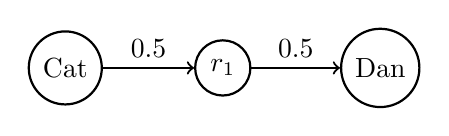
\begin{tikzpicture}[node distance={2cm}, thick, main/.style = {draw, circle}] 
    \node[main] (1) {\cn{Cat}}; 
    \node[main] (2) [right of=1] {$r_1$};
    \node[main] (3) [right of=2] {\cn{Dan}};
    \draw[->] (1) -- node[midway, above] {0.5} (2); 
    \draw[->] (2) -- node[midway, above] {0.5} (3);  
    \end{tikzpicture}
    \caption{Cat too Dan}
    \label{fig:y equals x}
\end{subfigure}
\hfill
 \begin{subfigure}[b]{0.4\textwidth}
     \centering
    \begin{tikzpicture}[node distance={2cm}, thick, main/.style = {draw, circle}] 
    \node[main] (5) [below of=2] {\cn{Ann}};
    \node[main] (6) [right of=5] {\cn{Bob}};
    \draw[->] (5) -- node[midway, below] {0.5} (6);
    % \draw[dashed] (2) -- (5);
    \end{tikzpicture}
    \caption{Cat to Dan \& Ann to Bob}
    \label{fig:y equals x}
\end{subfigure}

\end{center}
\caption{Example Path Connectivity }
  \label{fig:examplepath}
\end{figure}
As in \Cref{sec:qamsyntax1}, QAM permits a quantum protocol semantics through the manipulation of configurations and rules describing the communicating, granting, and cleaning steps for framing quantum network communications.
Here, we extend the configuration and rules in \Cref{fig:q-pi-semantics2} to define two important properties appearing in almost all quantum network protocols: connectivity and time.
The former refers to that quantum messages are always transmitted based on a connectivity graph, i.e., two cells can communicate if they have an edge in the graph and each edge has a certain success rate of message transmission. One example connectivity is in \Cref{fig:examplepath}.
The latter means that quantum messages are time-sensitive and are required to deliver in a short lifetime; otherwise, the messages are decohered and lost.

To define the two properties, we extend the configuration with the \cn{gt} and \cn{rel} cells in \Cref{fig:q-pi-semantics3},
which respectively contain a global clock time $t$ and a multiset of relation triples $R$ whose element is a triple of source and target cell locations and the success rate to transmit a message from the source to the target.
A user defined validity check function $f$ is used to determine if a message spends too much time in its transmission.
\Cref{fig:q-pi-semantics3} shows the semantic rule definitions for the two properties. Rule \rulelab{PC} is marked blue because it keeps the same as the case in \Cref{fig:q-pi-semantics2}, while the other rules require some modifications, explained below.
 
\noindent\textbf{Defining connectivity.}
Definition the property requires the update of rule \rulelab{GC} to \rulelab{GC1} in \Cref{fig:q-pi-semantics3}
by including the extra \cn{rel} cell.
In each message ($\qsend{p}{c}{m}^t$) transmission, we pattern match the source $c_1$ and target $c_1$ locations in the \cn{rel} cell as $(c_1,c_2,p')$. After the message is transmitted, we reduce its success rate as $p\cn{*}p'$, referring to that the message transmission results in a success rate reduction.

\noindent\textbf{Defining time.}
Definition this property is essentially two procedures.
First, a global time clock is introduced in the cell \cn{gt}.
In the upgraded rules (\rulelab{FC1} and \rulelab{AC1}) for cleaning steps, we include the \cn{gt} cell and increments the clock ($t\cn{+}$). We also include a new rule \rulelab{CT} to generate time stamp label for a message, so that we can mark the sending time of the message correctly. Second, we need to define a new granting rule by applying the validity check function $f$ to verify if a message's delivery is past due. To do so, we split the granting rule (\rulelab{Grant} in \Cref{fig:q-pi-semantics2}) into two rules.
For the case of message transmission (flag $c_1 \rightarrow c_2$ in \cn{comm}), it keeps the same;
otherwise, we apply function $f$ on a pair of time stamps, indicating the starting time of the message ($t$) and the final delivery time ($t'$), respectively. Function $f$ is user-defined. One example definition could be a lambda abstraction $\lambda\,(t,t')\,.\,t'-t<m$, where $m$ is a threshold time period for a message guaranteeing to deliver.

\begin{figure}[t]
{\footnotesize
\[\hspace*{-1em}
\begin{array}{lll}
&
\pcellb{\qsend{1}{c}{m}.0}{10}{\cn{Cat}}
\pcellb{0}{10}{r_1}
\pcellb{\qrev{c}{x}.0}{10}{\cn{Dan}} 
\qcellb{\emptyset}{\cn{comm}}
\qcellb{\texttt{F}}{\cn{pred}}
\qcellb{R}{\cn{rel}}
\qcellb{0}{\cn{gt}}
&
\\[0.3em]
\longrightarrow
&
\pcellb{\qsend{1}{c}{m}^0.0}{10}{\cn{Cat}}
\pcellb{0}{10}{r_1}
\pcellb{\qrev{c}{x}.0}{10}{\cn{Dan}} 
\qcellb{\emptyset}{\cn{comm}}
\qcellb{\texttt{F}}{\cn{pred}}
\qcellb{R}{\cn{rel}}
\qcellb{0}{\cn{gt}}
&
(\rulelab{CT})
\\[0.3em]
\longrightarrow
&
\pcellb{0}{9}{\cn{Cat}}
\pcellb{\qsend{0.5}{c}{m}^0.0}{9}{r_1}
\pcellb{\qrev{c}{x}.0}{10}{\cn{Dan}} 
\pcellb{(1.c.m)^0}{\cn{Cat}\rightarrow r_1}{\cn{comm}}
\qcellb{\texttt{F}}{\cn{pred}}
\qcellb{R}{\cn{rel}}
\qcellb{0}{\cn{gt}}
&
(\rulelab{GC1})
\\[0.3em]
\longrightarrow
&
\pcellb{0}{9}{\cn{Cat}}
\pcellb{\qsend{0.5}{c}{m}^0.0}{9}{r_1}
\pcellb{\qrev{c}{x}.0}{10}{\cn{Dan}} 
\pcellb{(1.c.m)^0}{\cn{Cat}\rightarrow r_1}{\cn{comm}}
\qcellb{\texttt{T}}{\cn{pred}}
\qcellb{R}{\cn{rel}}
\qcellb{0}{\cn{gt}}
&
(\rulelab{Grant1})
\\[0.3em]
\longrightarrow
&
\pcellb{0}{9}{\cn{Cat}}
\pcellb{\qsend{0.5}{c}{m}^0.0}{9}{r_1}
\pcellb{\qrev{c}{x}.0}{10}{\cn{Dan}} 
\qcellb{\emptyset}{\cn{comm}}
\qcellb{\texttt{F}}{\cn{pred}}
\qcellb{R}{\cn{rel}}
\qcellb{1}{\cn{gt}}
&
(\rulelab{FC1})
\\[0.3em]
\longrightarrow ...
\\[0.3em]
\longrightarrow
&
\pcellb{0}{9}{\cn{Cat}}
\pcellb{0}{8}{r_1}
\pcellb{\pard{\qsend{0.25}{c}{m}^0.0}{\qrev{c}{x}.0}}{9}{\cn{Dan}} 
\qcellb{\emptyset}{\cn{comm}}
\qcellb{\texttt{F}}{\cn{pred}}
\qcellb{R}{\cn{rel}}
\qcellb{2}{\cn{gt}}
&
\\[0.3em]
\longrightarrow
&
\pcellb{0}{9}{\cn{Cat}}
\pcellb{0}{8}{r_1}
\pcellb{0}{9}{\cn{Dan}} 
\pcellb{(0.25.c.m)^0}{\cn{Dan}}{\cn{comm}}
\qcellb{\texttt{F}}{\cn{pred}}
\qcellb{R}{\cn{rel}}
\qcellb{2}{\cn{gt}}
&
(\rulelab{Com},\rulelab{PC1})
\\[0.3em]
\longrightarrow
&
\pcellb{0}{9}{\cn{Cat}}
\pcellb{0}{8}{r_1}
\pcellb{0}{9}{\cn{Dan}} 
\pcellb{(0.25.c.m)^0}{\cn{Dan}}{\cn{comm}}
\qcellb{f(0,2)}{\cn{pred}}
\qcellb{R}{\cn{rel}}
\qcellb{2}{\cn{gt}}
&
(\rulelab{Grant2})
\\[0.3em]
\xrightarrow{0.25.c.m}&
\pcellb{0}{9}{\cn{Cat}}
\pcellb{0}{8}{r_1}
\pcellb{0}{9}{\cn{Dan}} 
\qcellb{\emptyset}{\cn{comm}}
\qcellb{\texttt{F}}{\cn{pred}}
\qcellb{R}{\cn{rel}}
\qcellb{3}{\cn{gt}}
&
(\rulelab{AC1})
\end{array}
\]
}
{\footnotesize
\begin{center}
$R\triangleq\{(\cn{Cat},r_1,0.5), (r_1,\cn{Dan},0.5)\}$
\qquad
$f=\lambda\,(t,t')\,.\,t'-t<5$
\end{center}
}
\caption{Example transitions based on the model in \Cref{fig:q-pi-semantics3}.}
  \label{fig:q-pi-example1}
\end{figure}


\Cref{fig:q-pi-example1} shows an example evaluation of the initial configuration on the top,
which is an instantiation of metavariables in configuration pattern in \Cref{fig:q-pi-semantics3}.
We first apply rule \rulelab{CT} to generate time stamp $0$ for the sending process action $\qsend{0.25}{c}{m}$.
We then apply rule \rulelab{GC1} and the two consecutive rules to transmit the action to cell $r_1$.
We can perform rule \rulelab{GC1} because the triple $(\cn{Cat},r_1,0.5)$ is in $R$.
During the steps, a piece of qubit resouce is consumed in both \cn{Cat} and $r_1$ cells, the action's success rate is reduced to $0.5$, and the global clock is updated to $1$.
After another round of message transmission steps, the action is conveyed to cell \cn{Dan}.
We then use rule \rulelab{PC}, with rule \rulelab{Com}, to deliver the action.
with the rule applications \rulelab{Grant2} and \rulelab{AC1} to grant and clean the delivery.
The delivery is granted, because the validity check results in $f(0,2)=2-0<5=\cn{T}$.

On the other hand, if users set the validity check function to be $\lambda\,(t,t')\,.\,t'-t<2$,
the validity check here results in $f(0,2)=2-0<2=\cn{F}$, which means that the evaluation is stuck at the \rulelab{Grant2} step.







